\documentclass[11pt, a4paper]{article}
\usepackage{pdfpages}
\usepackage{parallel}
\usepackage[T2A]{fontenc}
%\usepackage{ucs}
\usepackage[utf8]{inputenc}
\usepackage[english,russian]{babel}
\usepackage{hyperref}
\usepackage{rotating}
\usepackage[inner=2cm,top=1.8cm,outer=2cm,bottom=2.3cm,nohead]{geometry}
%\usepackage{listings}
\usepackage{graphicx}
\usepackage{wrapfig}
\usepackage{longtable}
\usepackage{indentfirst}
\usepackage{array}
\usepackage{tikzsymbols}
\usepackage{soul}
\usepackage[ruled,vlined]{algorithm2e}
\usepackage{qrcode}
\counterwithout{figure}{section} 

\usepackage{url}
\makeatletter
\g@addto@macro{\UrlBreaks}{\UrlOrds}
\makeatother

\newcolumntype{P}[1]{>{\raggedright\arraybackslash}p{#1}}
\frenchspacing
%\usepackage{fixltx2e} %text sub- and superscripts
\usepackage{icomma} % коскі ў матэматычным рэжыме
%\PreloadUnicodePage{4}

\newcommand{\longpage}{\enlargethispage{\baselineskip}}
\newcommand{\shortpage}{\enlargethispage{-\baselineskip}}

\def\switchlang#1{\expandafter\csname switchlang#1\endcsname}
\def\switchlangbe{
\let\saverefname=\refname%
\def\refname{Літаратура}%
\def\figurename{Іл.}%
}
\def\switchlangru{
\let\saverefname=\refname%
\let\savefigurename=\figurename%
\def\refname{Литература}%
\def\figurename{Рис.}%
}
\def\switchlangen{
\let\saverefname=\refname%
\def\refname{References}%
\def\figurename{Fig.}%
}

\hyphenation{admi-ni-stra-tive}
\hyphenation{ex-pe-ri-ence}
\hyphenation{fle-xi-bi-li-ty}
\hyphenation{Py-thon}
\hyphenation{ma-the-ma-ti-cal}
\hyphenation{re-ported}
\hyphenation{imp-le-menta-tions}
\hyphenation{pro-vides}
\hyphenation{en-gi-neering}
\hyphenation{com-pa-ti-bi-li-ty}
\hyphenation{im-pos-sible}
\hyphenation{desk-top}
\hyphenation{elec-tro-nic}
\hyphenation{com-pa-ny}
\hyphenation{de-ve-lop-ment}
\hyphenation{de-ve-loping}
\hyphenation{de-ve-lop}
\hyphenation{da-ta-ba-se}
\hyphenation{plat-forms}
\hyphenation{or-ga-ni-za-tion}
\hyphenation{pro-gramming}
\hyphenation{in-stru-ments}
\hyphenation{Li-nux}
\hyphenation{sour-ce}
\hyphenation{en-vi-ron-ment}
\hyphenation{Te-le-pathy}
\hyphenation{Li-nux-ov-ka}
\hyphenation{Open-BSD}
\hyphenation{Free-BSD}
\hyphenation{men-ti-on-ed}
\hyphenation{app-li-ca-tion}

\def\progref!#1!{\texttt{#1}}
\renewcommand{\arraystretch}{2} %Іначай формулы ў матрыцы зліпаюцца з лініямі
\usepackage{array}

\def\interview #1 (#2), #3, #4, #5\par{

\section[#1, #3, #4]{#1 -- #3, #4}
\def\qname{LVEE}
\def\aname{#1}
\def\q ##1\par{{\noindent \bf \qname: ##1 }\par}
\def\a{{\noindent \bf \aname: } \def\qname{L}\def\aname{#2}}
}

\def\interview* #1 (#2), #3, #4, #5\par{

\section*{#1\\{\small\rm #3, #4. #5}}
\ifx\ParallelWhichBox\undefined%
    \addcontentsline{toc}{section}{#1, #3, #4}%
\else%
\ifnum\ParallelWhichBox=0%
    \addcontentsline{toc}{section}{#1, #3, #4}%
\fi\fi%

\def\qname{LVEE}
\def\aname{#1}
\def\q ##1\par{{\noindent \bf \qname: ##1 }\par}
\def\a{{\noindent \bf \aname: } \def\qname{L}\def\aname{#2}}
}

\newcommand{\interviewfooter}[1]{
\vskip 1em
\noindent \textit{#1}
}

\AtEndDocument{\vfill\centering \qrcode{https://github.com/fiowro/mouses/blob/main/\jobname.pdf}}

\switchlang{en}
\begin{document}

\title{1984 -- Mindset Mouse}
\date{}
\maketitle
\selectlanguage{english}

Mindset Mouse came bundled with the Mindset personal computer. The Mindset computer was released in 1984 by Mindset Corporation, and was on sale for only a year. In technical terms, it was partially compatible with the IBM PC, based on the Intel 80186 processor and a non-standard graphics subsystem that had enhanced capabilities, including hardware acceleration of some typical graphics operations \cite{byteMagazine}.

The real manufacturer of the mouse was the Japanese company Alps -- the manufacturer of the first Japanese mouse, MZ-1X10, introduced to the Japanese market one year earlier.

\begin{figure}[h]
   \centering
    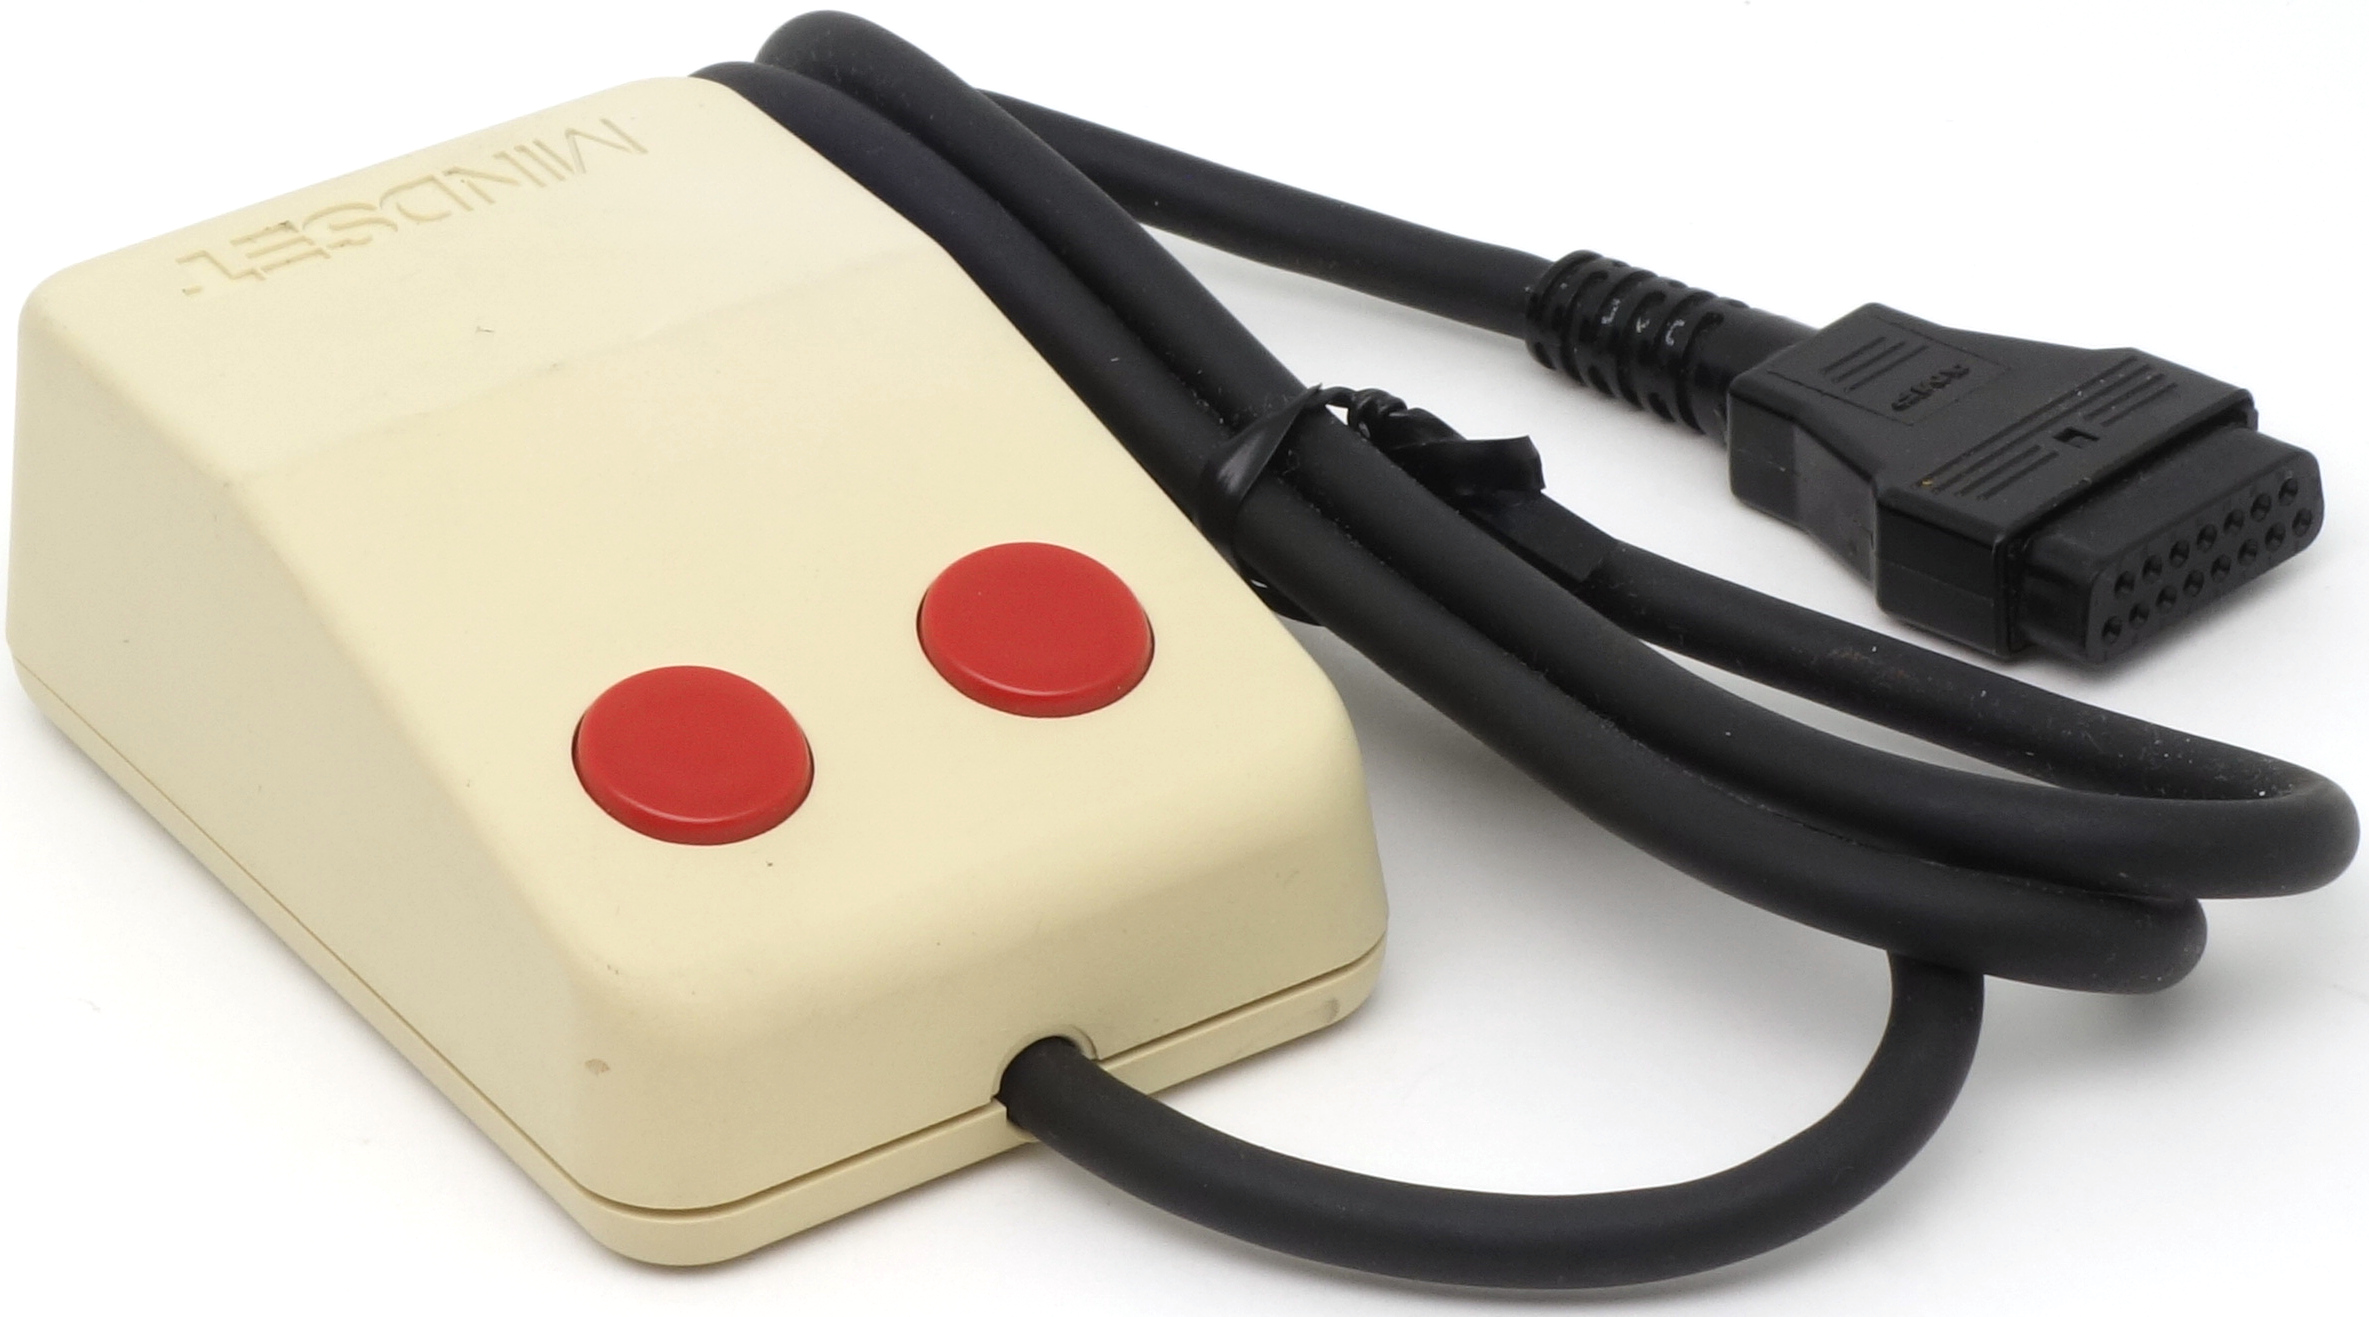
\includegraphics[scale=0.6]{1984_mindset_mouse/pic_30.jpg}
    \caption{Mindset Mouse}
    \label{fig:MindsetMousePic}
\end{figure}

The mouse body is a beige parallelepiped with slightly rounded edges and a wedge-shaped cut of the upper part of the body, on which there is a pair of round red buttons (fig. \ref{fig:MindsetMousePic}). Thanks to these unusual contrasting buttons, Mindset Mouse has a memorable look and therefore is constantly present in advertising materials for Mindset computers \cite{adv}.

\begin{figure}[h]
    \centering
    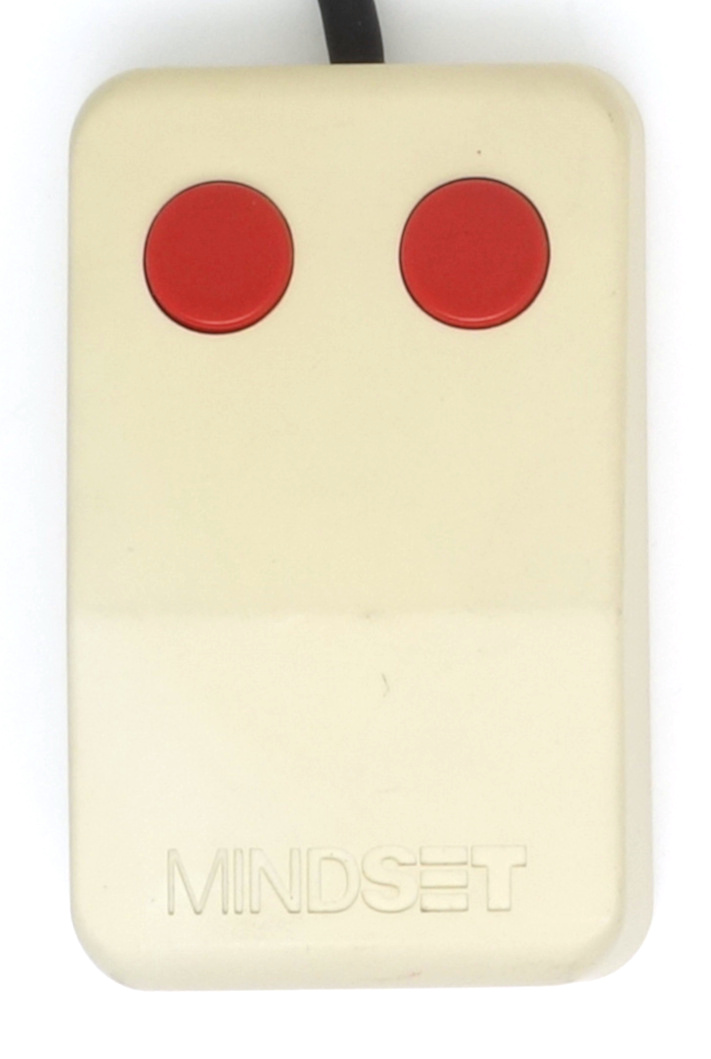
\includegraphics[scale=0.6]{1984_mindset_mouse/top_30.jpg}
    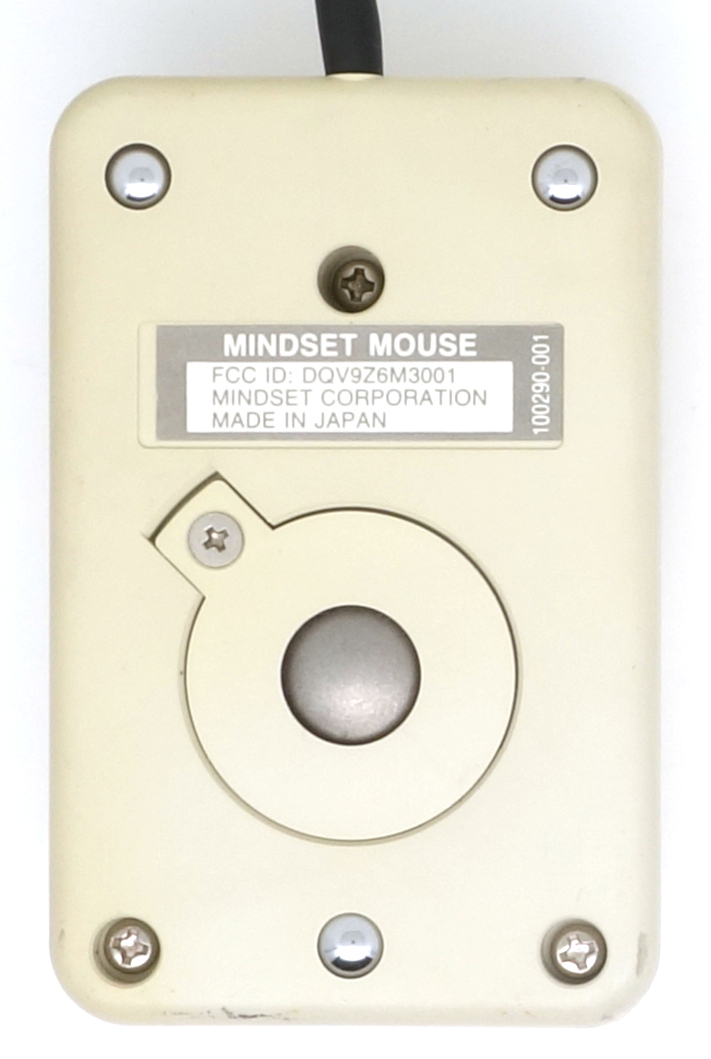
\includegraphics[scale=0.6]{1984_mindset_mouse/bottom_30.jpg}
    \caption{Mindset Mouse, top and bottom views}
    \label{fig:MindsetMouseTopAndBottom}
\end{figure}

The underside of the mouse is similar to the MZ-1X10, showing off a heavy steel ball and three small, smooth-polished balls act as feet to minimize friction. Also, a removable ring is provided in the bottom of the case, which allows you to remove the ball and get rid of the collected debris; however, the snap ring option has not yet been invented, so it must be unscrewed with a screwdriver. The design does not provide protection for the wire from damage at the point where it exits the mouse body, since at the time the mouse was released its need was not yet obvious (fig. \ref{fig:SharpMZ1x10TopAndBottom}).

\begin{figure}[h]
    \centering
    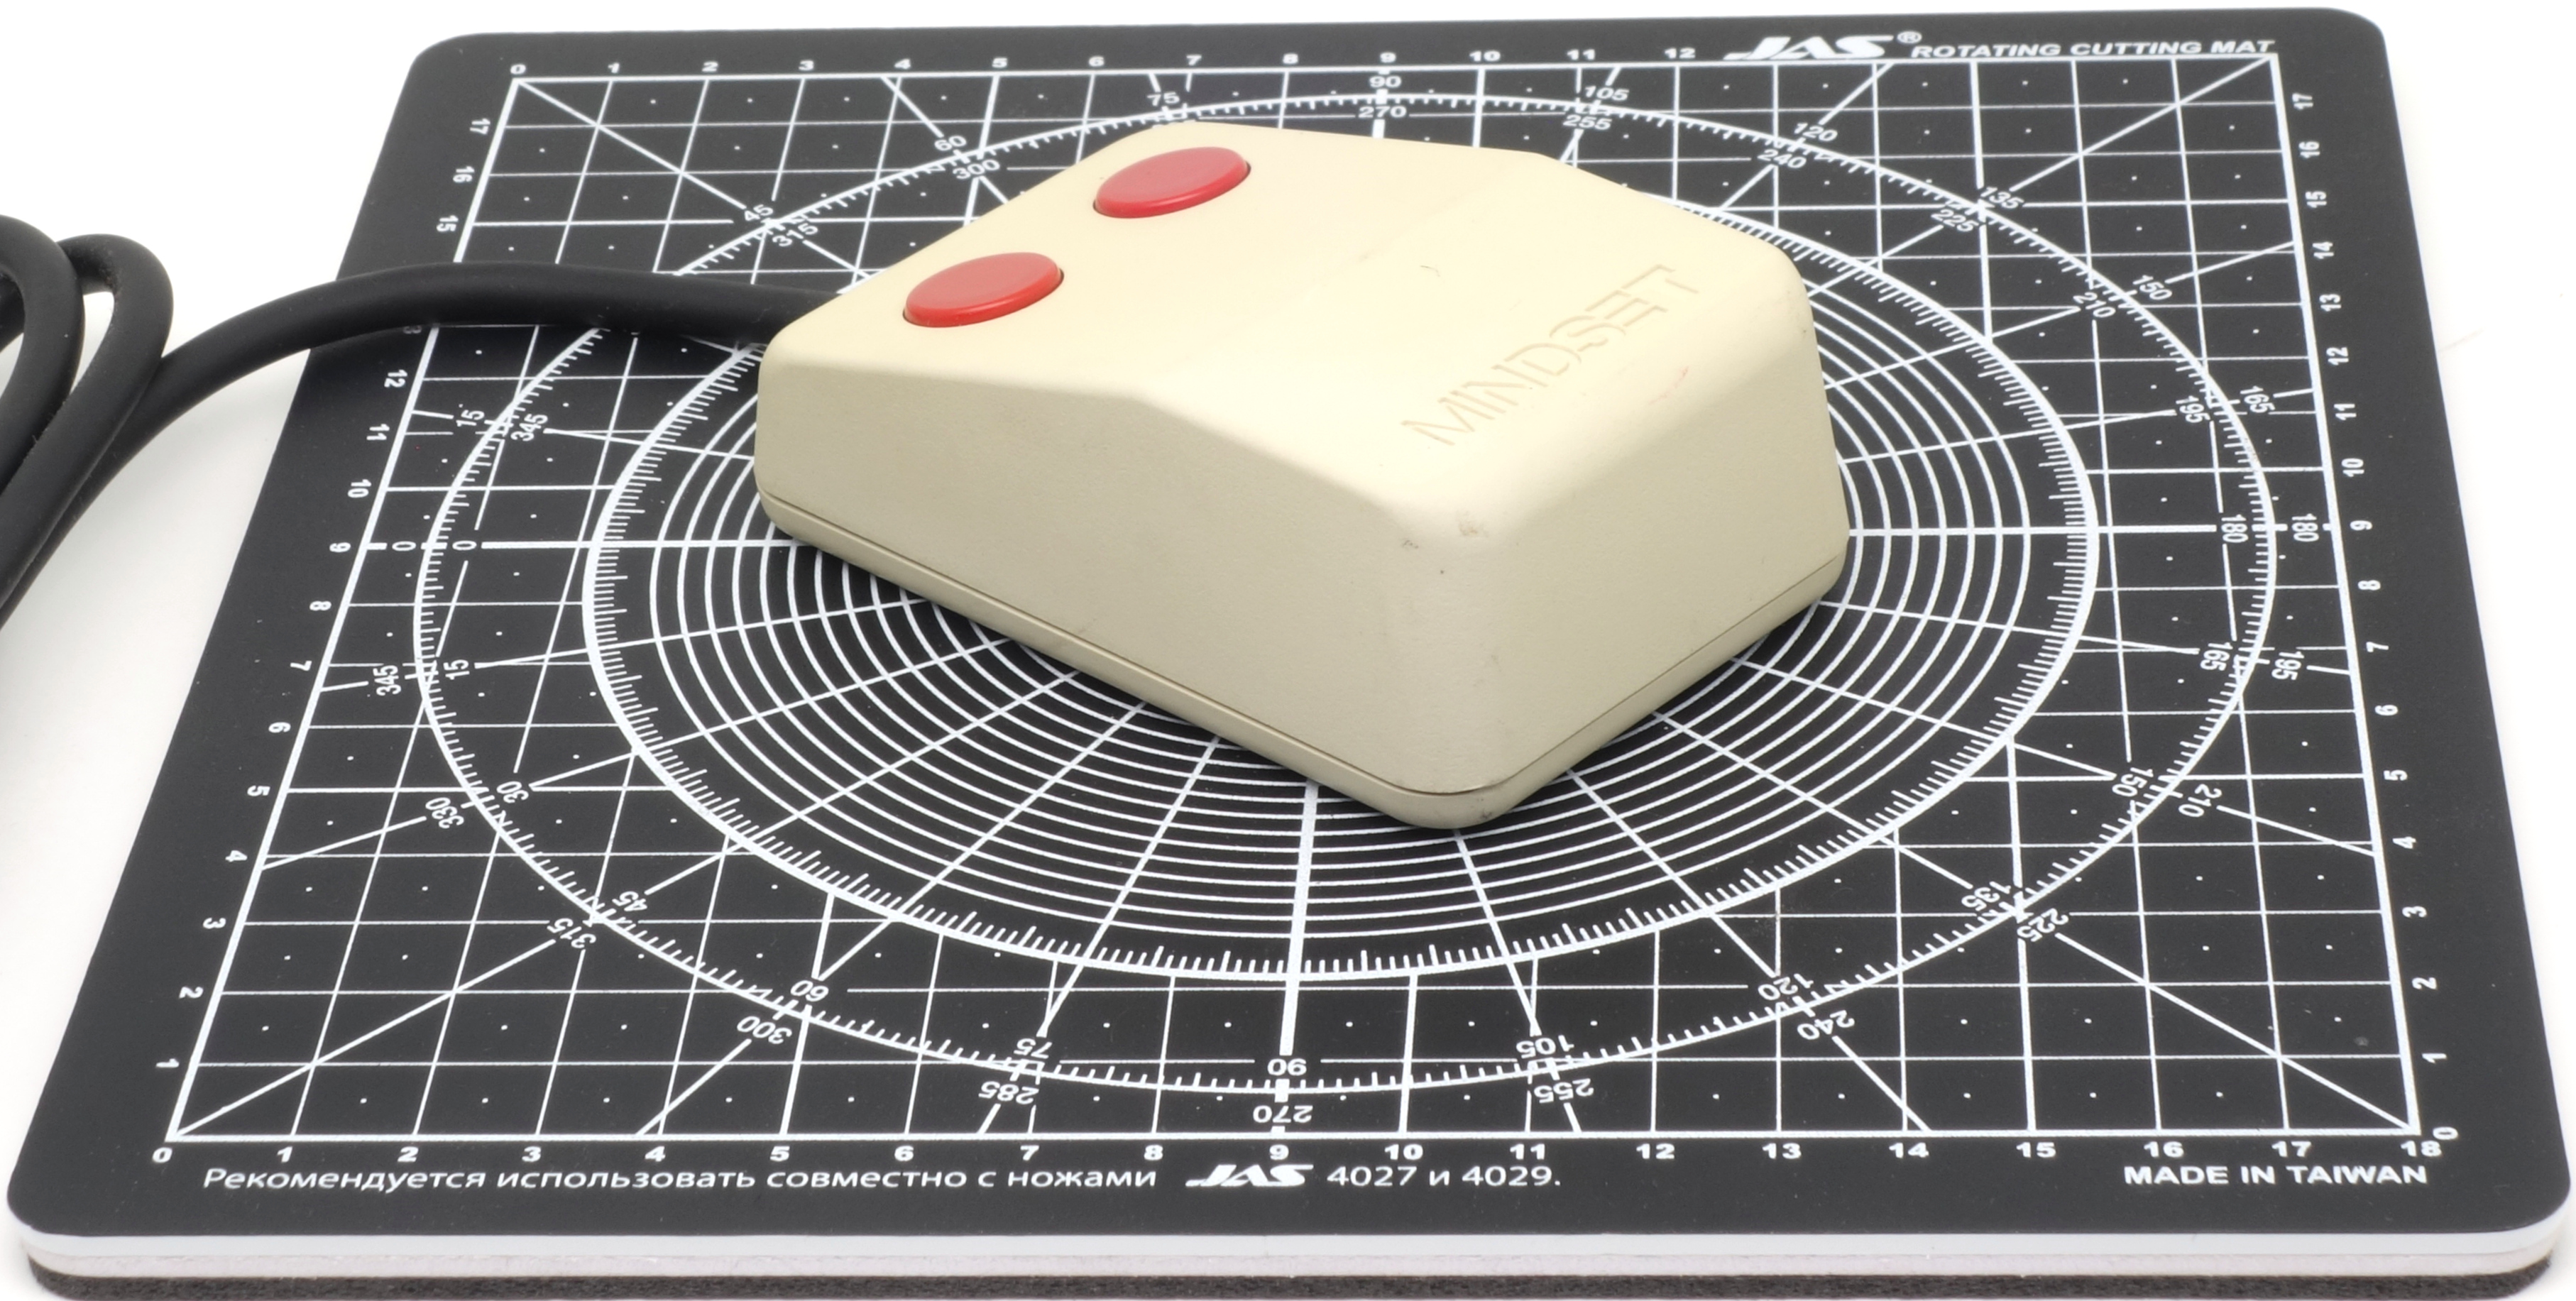
\includegraphics[scale=0.5]{1984_mindset_mouse/size_15.jpg}
    \caption{Mindset Mouse on a graduated pad with a grid step of 1~cm}
    \label{fig:MindsetMouseSize}
\end{figure}

The already small size of the mouse (fig. \ref{fig:MindsetMouseSize}) seems even smaller due to the wedge-shaped body (the inclined part occupies two-thirds of its length), but the mouse is quite heavy. The developers' desire to achieve an impressive design did not have the best effect on ergonomics. The buttons are small and not in the most ideal position (they are located some distance from the edge of the body, which affects the way the palm grips the mouse). The edge of the case closest to the user is almost vertical, but even if it were inclined, taking into account the size of the mouse, this would not make significant improvements in ease of use (fig. \ref{fig:SharpMZ1x10Hand}).

\begin{figure}[h]
    \centering
    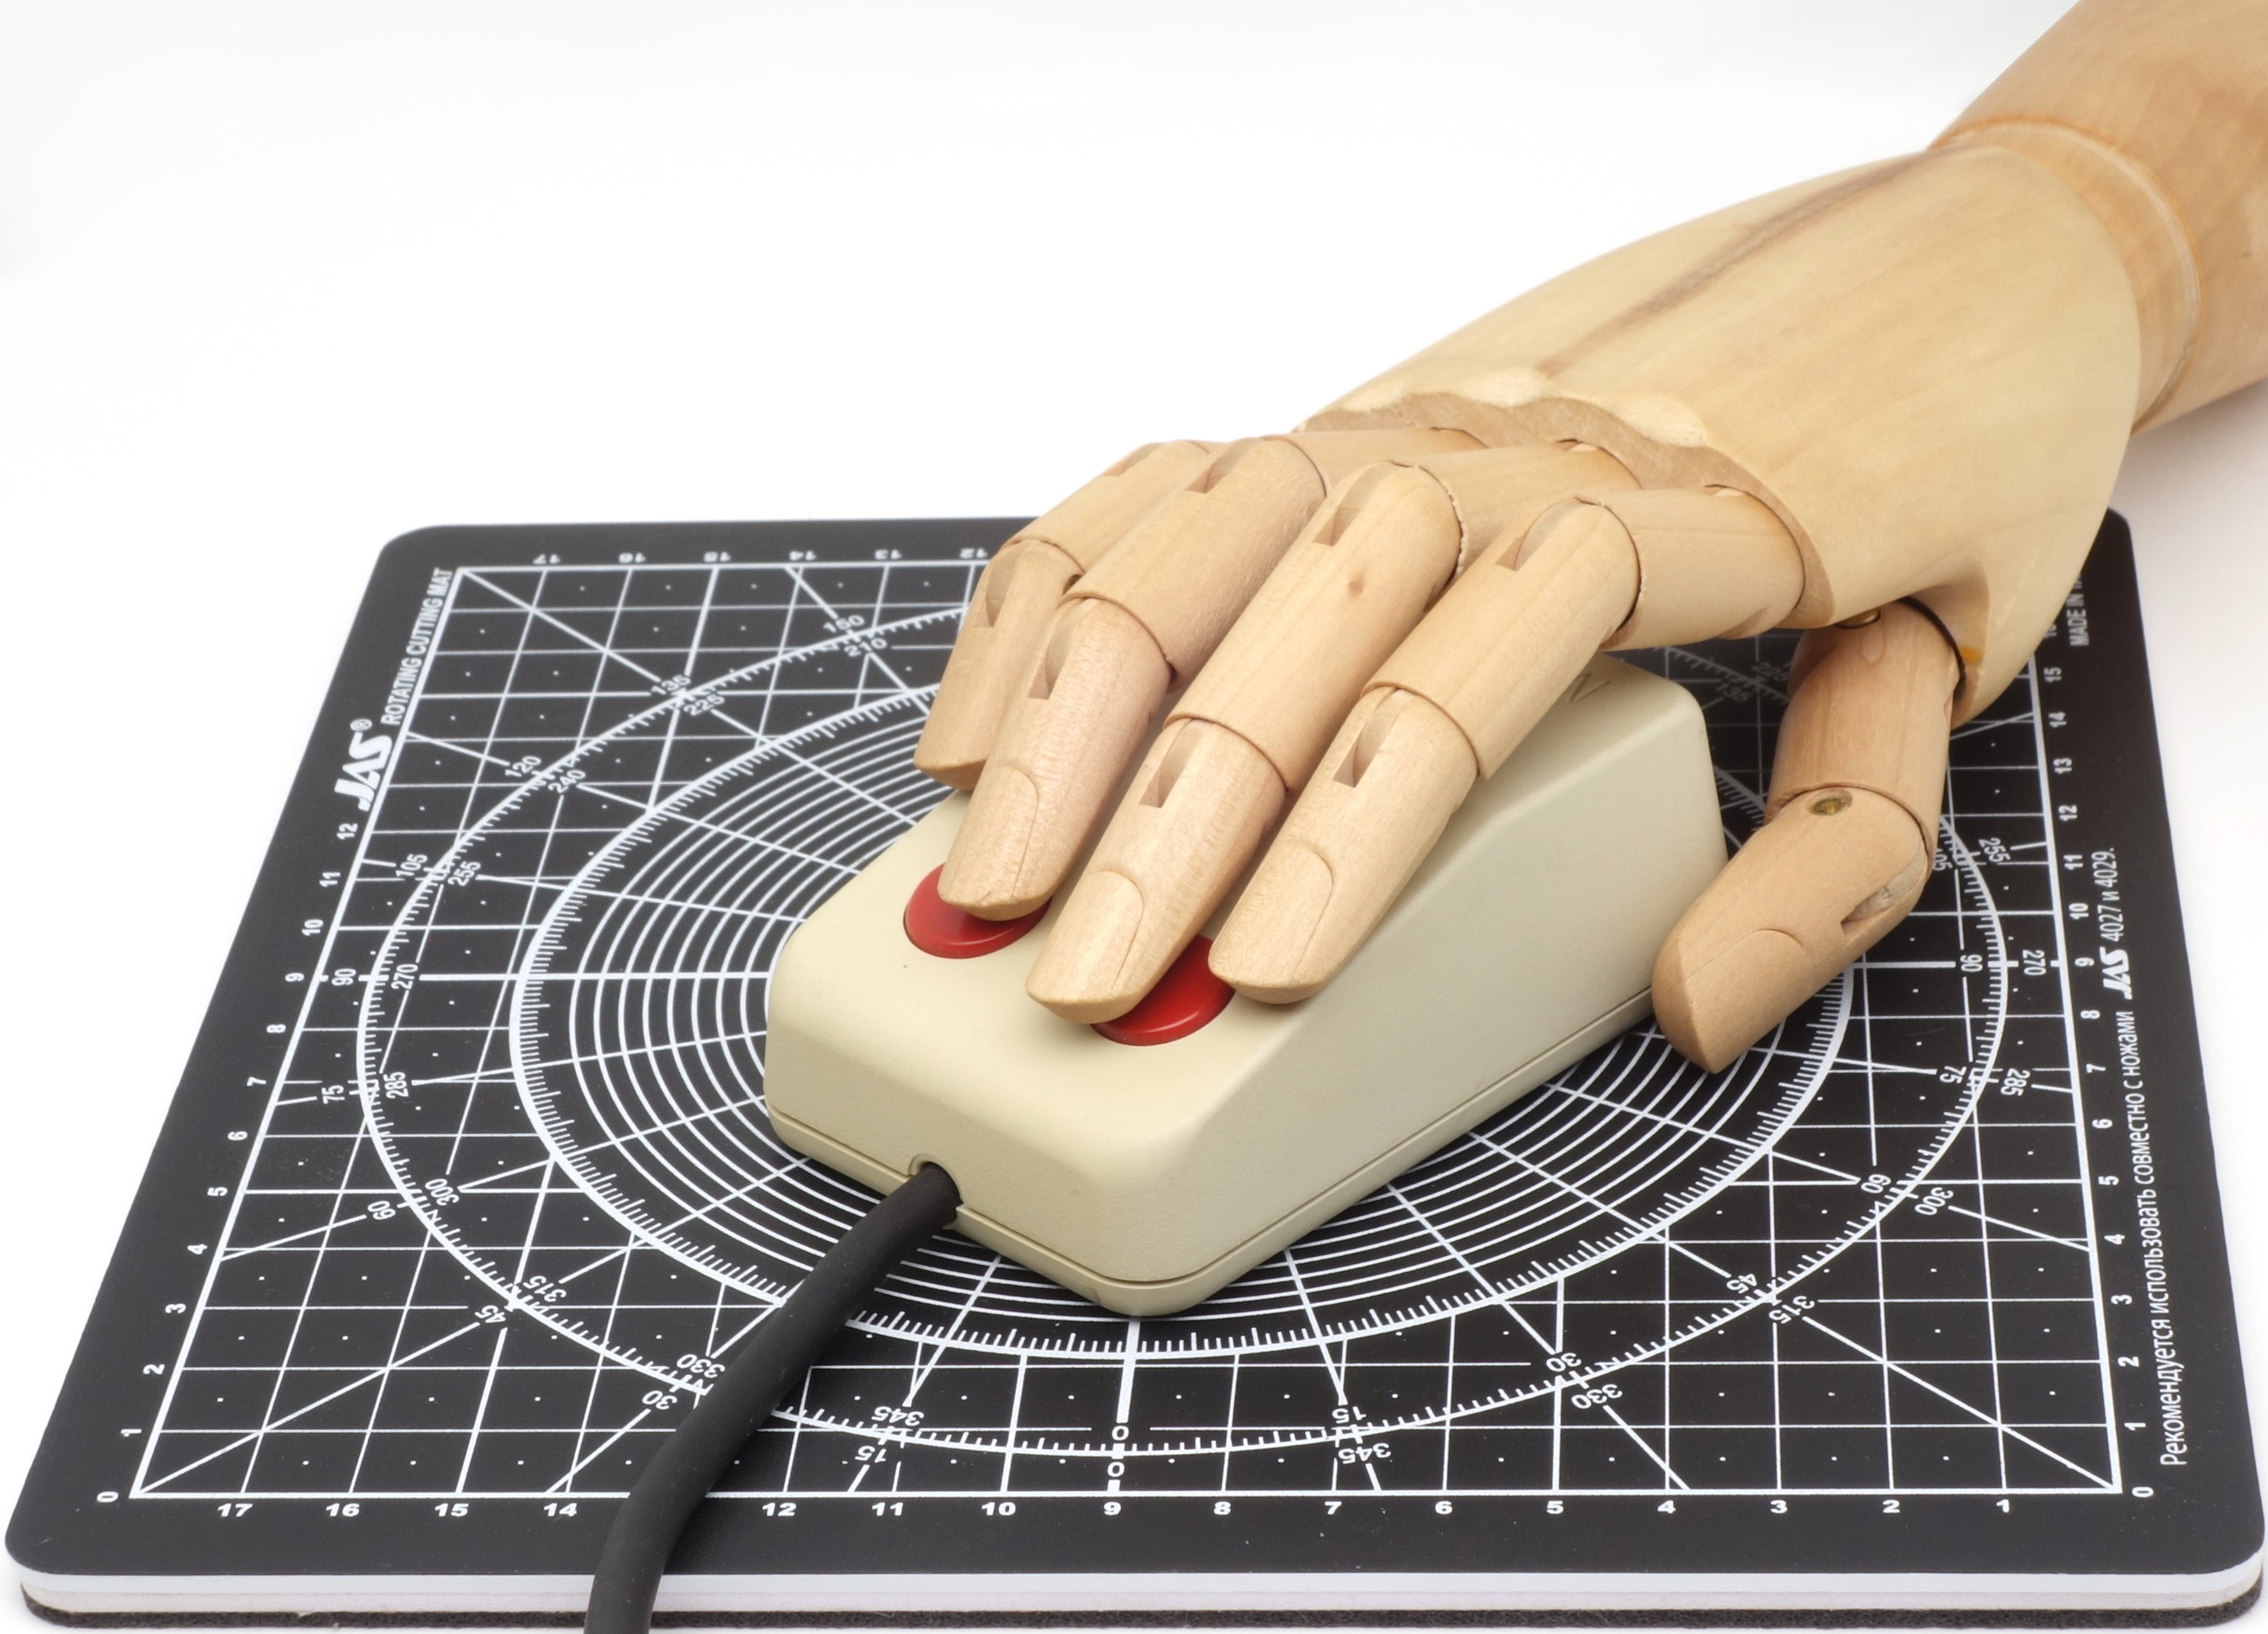
\includegraphics[scale=0.5]{1984_mindset_mouse/hand_30.jpg}
    \caption{Mindset Mouse with a human hand model}
    \label{fig:MindsetMouseHand}
\end{figure}

The internal structure of the mouse can be seen in fig. \ref{fig:MindsetMouseInside}. The mouse uses the design of the first generation Alps mice based on closed contact encoders. When compared with other products based on this design -- the MZ-1X10 mouse and the first Microsoft mouse -- the design is almost completely identical, with the exception of the configuration of boards and elements associated with different mouse connection interfaces.

 \begin{figure}[h]
    \centering
    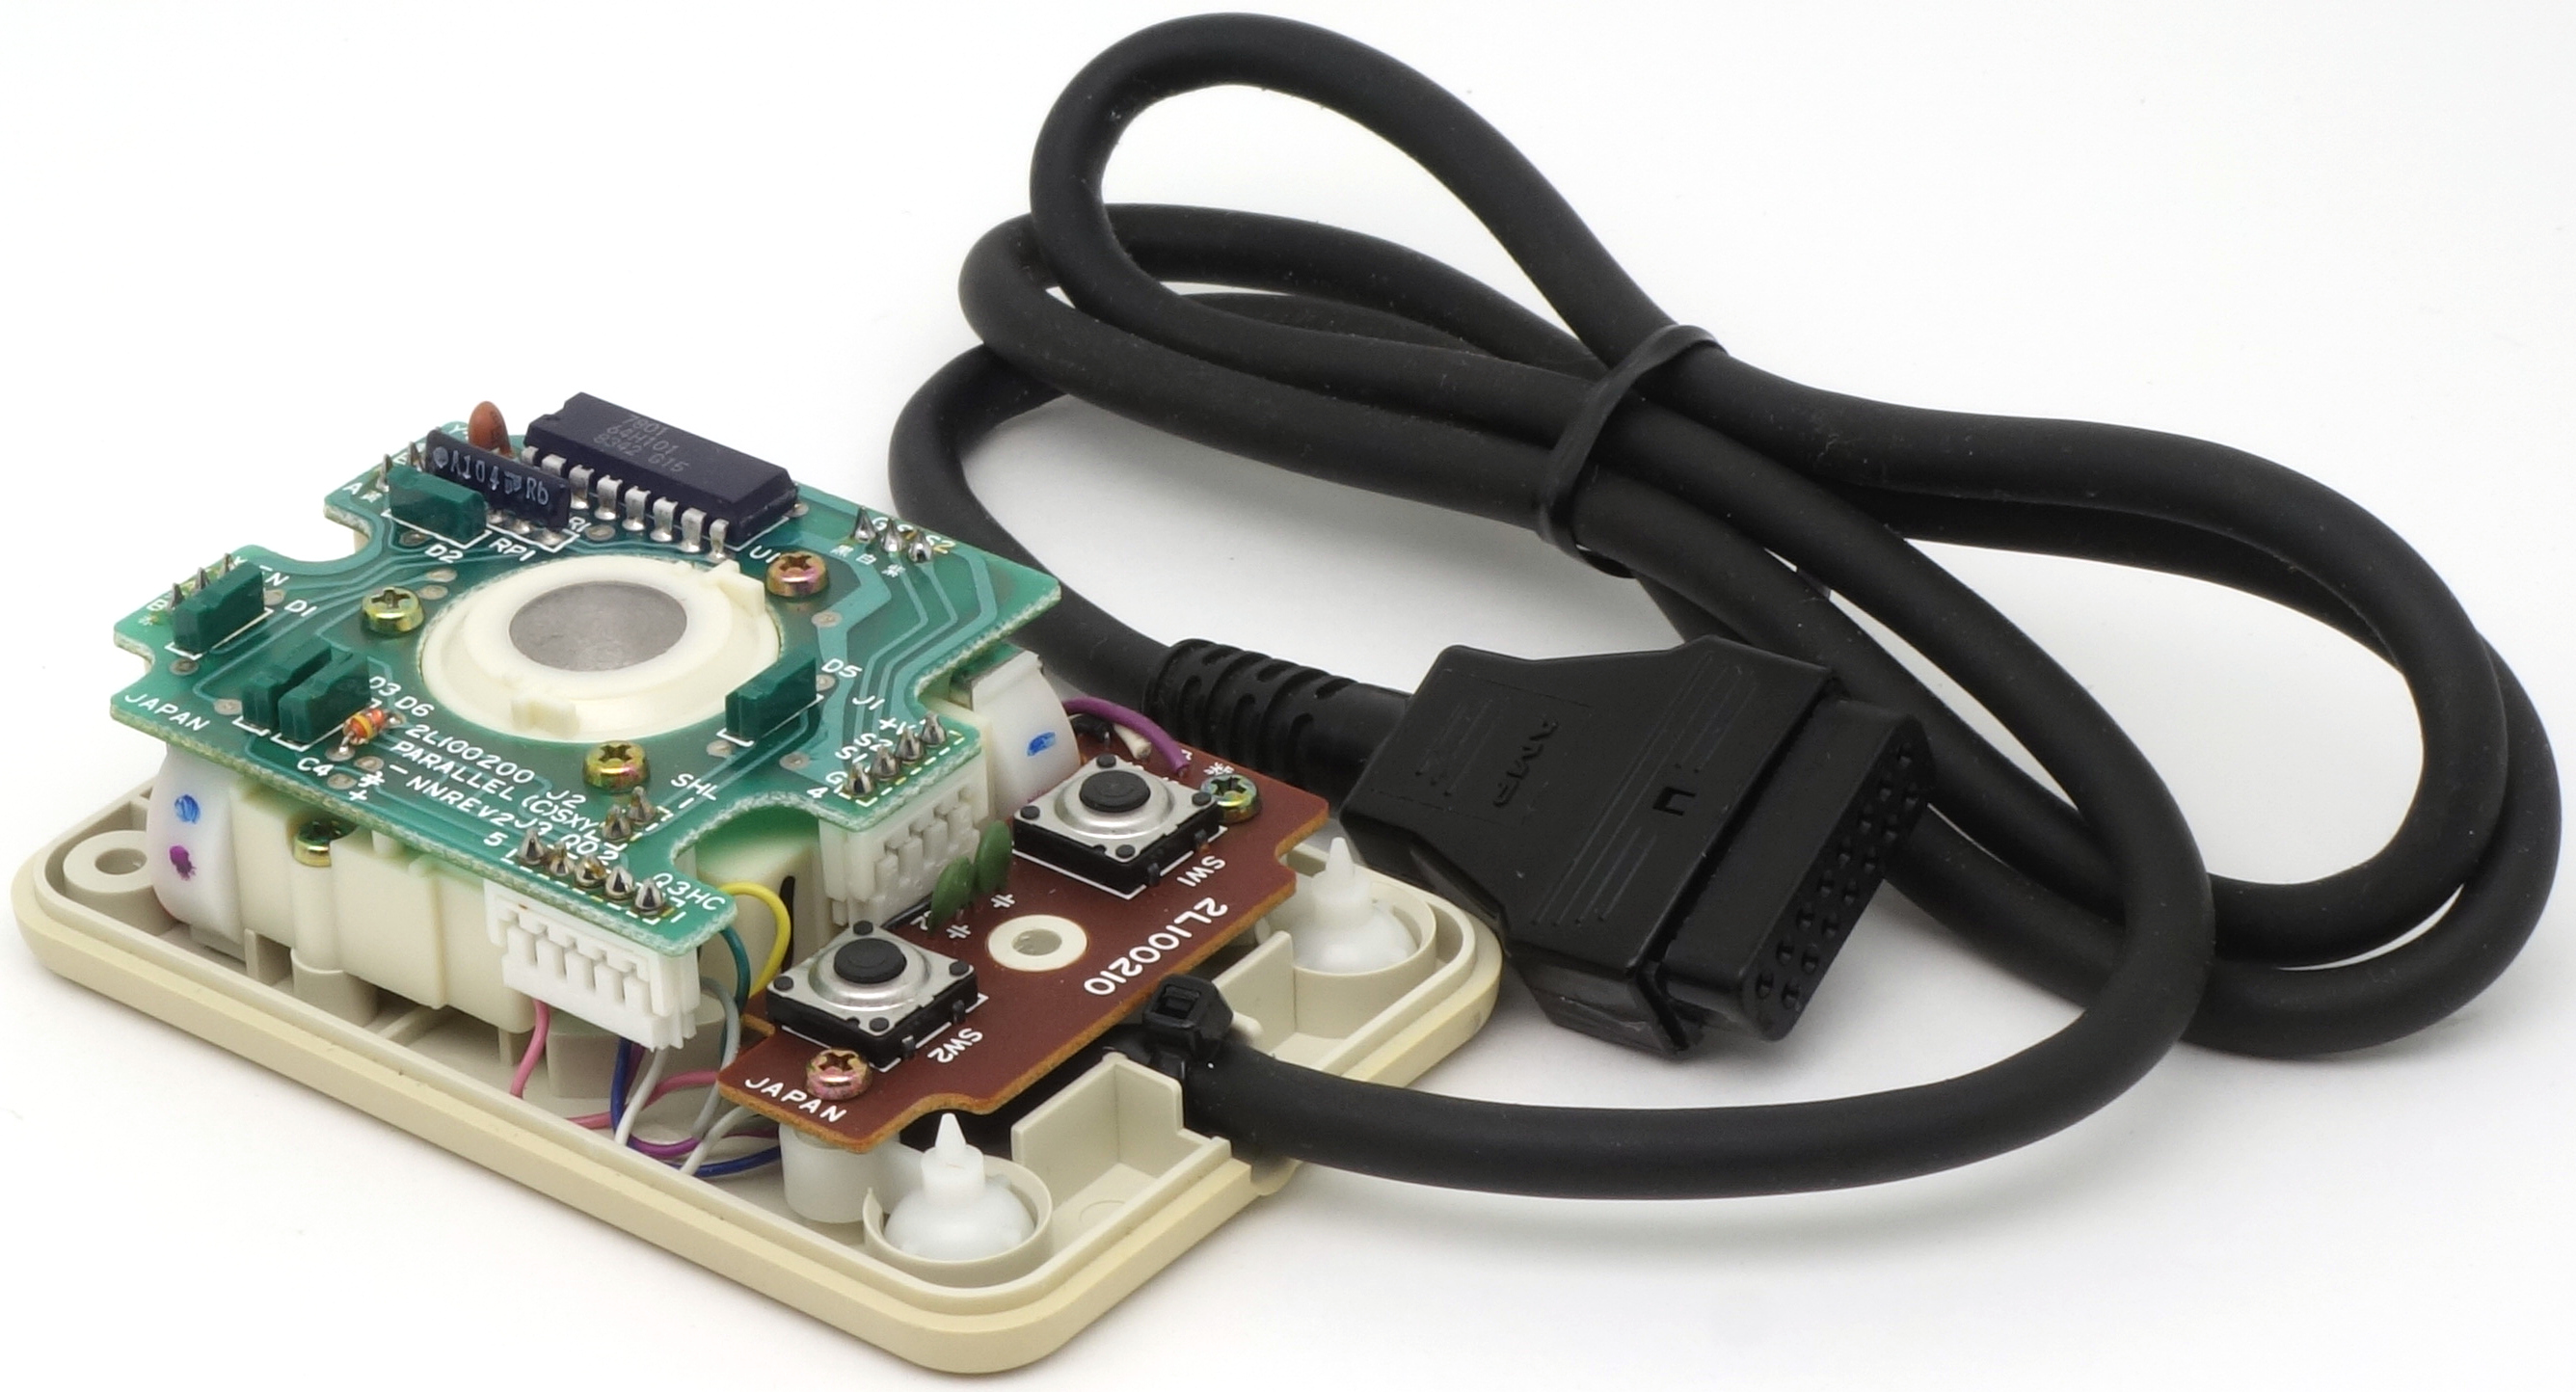
\includegraphics[scale=1]{1984_mindset_mouse/inside_30.jpg}
    \caption{Mindset Mouse disassembled}
    \label{fig:MindsetMouseInside}
\end{figure}

\begin{thebibliography}{9}
\bibitem {byteMagazine} Wadlow T. The Mindset Personal Computer // Byte Magazine, Vol. 10, No. 6. June, 1985. - P. 324-232 \url{https://archive.org/details/byte-magazine-1985-06/page/n331/mode/2up}
\bibitem{adv} Mindset Personal Computer System \url{https://archive.org/details/bitsavers_mindsetBrore_3744143/page/n1/mode/2up}
\end{thebibliography}
\end{document}
